\documentclass{article} % for thesis

% \usepackage[top=0.5in, bottom=0.5in, left=0.5in, right=0.5in]{geometry}
% \documentclass[twocolumn,9pt]{article}
\usepackage{spconf}
\usepackage[utf8]{inputenc}
\usepackage{natbib}
\usepackage{graphicx}
\usepackage{stfloats} % for positioning of figure* on the same page
\usepackage{caption}
\usepackage{tikz}
\usepackage[inline]{enumitem}
\usepackage{amsmath}
\usepackage{subcaption}
\usepackage[breaklinks=true,colorlinks=true, allcolors=blue]{hyperref}
\usepackage{breakcites}
\usepackage{microtype}
\usepackage{lipsum}
\usepackage{xcolor}
\usepackage{array}
\usepackage{float}
\usepackage{adjustbox}
\usepackage{listings}
\usepackage{csquotes}
\usepackage{makecell}
\usepackage{pdfpages}
\usepackage{xspace}
\usepackage{tikz}
\usetikzlibrary{positioning,shapes.geometric}

% to do:
% a few more scenarios
% hearing tests
% one other way to present results is grouped by which losses are most appropriate for each situtation

\usepackage{xcolor}
\usepackage[utf8]{inputenc}       % For UTF-8 encoding
\usepackage{listings}
\usepackage{amsmath}              % Optional: for math symbols
\usepackage{anyfontsize}
\usepackage{graphicx} % required for \scalebox

\lstdefinelanguage{Faust}{
    morekeywords={import, process, environment, declare, with, if, else, while, for, int, float, true, false},
    sensitive=true,
    morecomment=[l]{//}, % Line comment
    morecomment=[s]{/*}{*/}, % Block comment
    morestring=[b]", % Strings
}

% Customize the appearance of the code
\lstset{
    language=Faust,
    backgroundcolor=\color{lightgray!20},
    % basicstyle=\ttfamily\small,
    basicstyle=\fontsize{8pt}{9pt}\selectfont\ttfamily,
    keywordstyle=\color{blue}\bfseries,
    stringstyle=\color{orange},
    commentstyle=\color{green}\itshape,
    showstringspaces=false,
    % numbers=left,
    % numberstyle=\tiny,
    frame=single,
    breaklines=true,
      % basicstyle=\ttfamily,
  % literate={\delta}{{\(\delta\)}},
}


\captionsetup[lstlisting]{justification=centering, singlelinecheck=false}
\providecommand{\gls}[1]{#1}
\newcommand{\highlight}[1]{\textcolor[RGB]{00,150,00}{#1}}
\newcommand{\todo}[1]{\textcolor{red}{#1}}

\newcommand{\SIMSESpec}{\texttt{SIMSE\_Spec}\xspace}
\newcommand{\LoneSpec}{\texttt{L1\_Spec}\xspace}
\newcommand{\JTFS}{\texttt{JTFS}\xspace}
\newcommand{\DTWEnv}{\texttt{DTW\_Envelope}\xspace}
\newcommand{\OutDomain}{\textbf{Out-of-Domain Generation}\xspace}
\newcommand{\LossSelect}{\textbf{Loss Selection}}
\newcommand{\SynthSelect}{\textbf{Synthesis Selection}}
\newcommand{\PeriodicLoss}{\textbf{Periodic Loss}}

\newcommand{\BPNoise}{\textbf{BP-Noise}\xspace}
\newcommand{\BPSaw}{\textbf{BP-Saw}\xspace}
\newcommand{\AddSineSaw}{\textbf{Add-SineSaw}\xspace}
\newcommand{\AmpMod}{\textbf{Noise-AM}\xspace}
\newcommand{\FMMod}{\textbf{SineSaw-AM}\xspace}
\newcommand{\FMModvtwo}{\textbf{SineSine-AM}\xspace}
\newcommand{\PitchBendUp}{\textbf{PitchBend-Up}\xspace}

\title{Selecting Loss Functions for Out-of-Domain Sound-Matching}
\begin{document}

% \author{Amir Salimi, Abram Hindle, Osmar R. Za{\"i}ane}

\name{Amir Salimi, Abram Hindle, Osmar R. Za{\"i}ane}
\address{University of Alberta}

\maketitle

\begin{abstract}
    Out-of-domain sound-matching refers to automatically programming a synthesizer towards a sound that it cannot accurately replicate. Measuring performance in out-of-domain sound-matching is a difficult task due reasons such as the subjective experience of sound, open-set recognition, etc. Here we present a series of out-of-domain tasks using four loss functions and synthesizers with non-overlapping functionalities. The experiments here are designed such that differences in parameters (whether all parameters or a subset) are well suited for measuring performance in sound-matching. The out-of-domain experiments here confirm that the success of loss functions is highly dependent on the method of synthesis and the target sound. 
\end{abstract}

\section{Introduction}
Audio synthesizers are musical instruments which utilize digital signal processing (DSP) functions for the creation of sound.  One method of sound-design with a synthesizer is approximating the characteristics of a desired (or target) sound with a synthesizer. This often requires the continual and iterative process of listening to the output of the synthesizer and modifying the parameters accordingly until satisfied. \textit{Sound-matching} is the term used for the automation of this process, which critically relies on automatic listening, i.e., a function for measuring similarity between the target sound and the output of the synthesizer. 

The are major areas of weakness in current literature that require further research~\cite{salimi2025soundmatching}. One such issue is the lack of experiments pertaining to \OutDomain, i.e., use of target sounds which the audio synthesizer cannot reproduce. The overwhelming majority of current sound-matching works showcase experiments where the target sound is the output of the synthesizer itself, the true parameters are known, and the goal is to replicate the exact same target sound. This is not a realistic simulation of the manual approach, where the target sound is all but guaranteed to be from another source (be it synthesized or manually recorded) and the goal is not the direct replication of the target sound, but the imitation of a subset of its characteristics.

Defining success in out-of-domain sound-matching is difficult, as it calls for loss functions that \textit{only} measure differences in the characteristics of interest, which in turn can render the de facto, non-specific state-of-the-art (SOTA) methods of audio comparison such as multi-scale spectrogram loss (MSS) ~\cite{engel2020ddsp} ineffective. In a previous work, we presented a comparison of four different loss functions and their efficacy in sound-matching pipelines utilizing four different methods of synthesis~\cite{salimi2025soundmatching}, and saw that different loss functions are appropriate for different methods of synthesis~\cite{salimi2025soundmatching}; like the majority of previous works in sound-matching, the experiments were in-domain. Here, we expand this work with a series of out-of-domain experiments where the synthesizer used to generate the target sounds are different from the one used for sound-matching. 

Parameter loss (or P-LOSS) has been frequently used in previous works for measuring success in sound-matching. Although P-Loss does not always match up with hearing tests, it is nontheless useful. Here, we define the original target synthesizers such that their functionalities partially overlap with the output synthesizer, in this way, the experiments are out-of-domain but partial P-LOSS is still available as a measure of success. 


% In a previous work, we presented a number of sound-matching experiments which suggest that the selection of the best performing loss functions for sound-matching is highly dependent on the method of synthesis~\cite{salimi2025soundmatching}. Much like the majority of previous works in sound-matching, the experiments were in-domain, that is, the synthesizer is capable of perfect replication of the target sound (usually, the target sound is made by the synthesizer itself). We noted the lack of out-of-domain experiments as a weakness not only in our previous work, but in the field of sound-matching as a whole. 

% Despite their critical role in sound-matching, the performance of different sound-similarity measures (or loss functions) under different circumstances has rarely been a topic of research. Should we be looking for a global sound-similarity measure, or is the choice of loss function a creative decision, much like the selection of a synthesizer?




\begin{figure}[ht]
    \centering
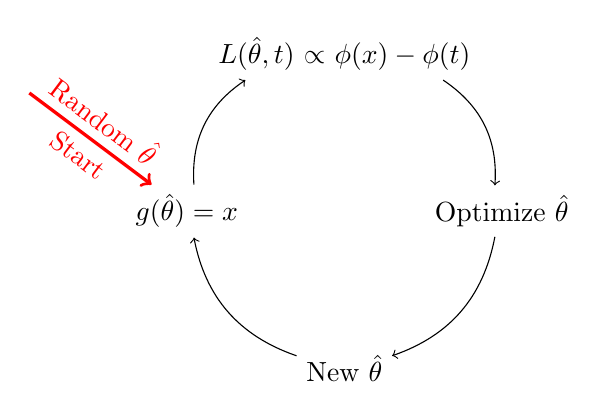
\begin{tikzpicture}[node distance=2cm, auto]

    % Nodes
    \node (start) [text centered] {\( g (\hat{\theta}) = x \)};
    \node (L) [above of=start,right of=start, text centered] {\( L(\hat{\theta},t) {\ \propto \ } \phi(x) - \phi(t) \)};
    \node (optimize) [below of=L,right of=L, text centered] {Optimize $\hat{\theta}$};
    \node (new_theta) [below of=optimize,right of = start, text centered] {New \( \hat{\theta} \)};

    % Highlight and arrow for the start node
    \draw[->, very thick, red] (start) ++(-2,1.5) -- (start)
        node[midway, below, align=center, sloped, color=red] {Start}
        node[midway, above, align=center, sloped, color=red] {Random $\hat{\theta}$};
        
    % Arrows with multi-line labels
    \draw[->, bend left] (start) to node[midway, right, align=center] {} (L);
    \draw[->, bend left] (L) to node[midway, right, align=center] {} (optimize);
    \draw[->, bend left] (optimize) to node[midway, below, align=center] {} (new_theta);
    \draw[->, bend left] (new_theta) to node[midway, left, align=center] {} (start);

\end{tikzpicture}
    \caption{ Iterative approach to sound design, as presented in~\cite{salimi2025soundmatching}}
    \label{fig:sound_design_loop_iterative}
\end{figure}

\section{Background}
All sound-matching works require a synthesizer, a loss function, and a method for determining the correct parameters. Iterative sound-matching uses a feedback loop similar to the manual approach. To paraphrase the formal definition given in previous works~\cite{salimi2025soundmatching,vahidi2023mesostructures,han2023perceptual}, a synthesizer $g$ with arbitrary (in this case, random) initialized parameters $\hat{\theta}$, creates sound $x$. The target sound $t$ is used as the goal. In-domain sound-matching implies that there exists a parameter set $\theta^*$ such that $g(\theta^*)$ is perceptually equal to $y$, where as out-of-domain sound-matching requires that there is no such set of parameters. In any case, the parameters $\hat{\theta}$ are adjusted to minimize error (or loss) $L(\hat{\theta},t)$, where $L$ is proportional to the difference between the representations of $x$ and $t$. $\phi$ is the audio feature extractor, or representation function, algorithms derived from Fourier transformations such as short-time Fourier transforms (STFT) or MSS are the most common form of $\phi$.

\subsection{Loss Functions}
In-domain experiments have shown that in a differentiable, iterative sound-matching setting, different loss functions appear to be appropriate for different methods of synthesis~\cite{salimi2025soundmatching}. This work is the further analysis of the interplay between the same loss functions and synthesizers in out-of-domain settings. 


\section{Experiment Setup}
\label{sec:experiment_setup}
% loss functions, target vs imitator, training loop
For each combination of synthesizer program and loss function, 300 sound-matching experiments are conducted and the automatic evaluation evaluation values are recorded after 200 iterations of the sound-matching loop. From the 300 targets and outputs, we select 40 examples for manual ranking. 


\section{Out-of-Domain Examples}
We look at some examples of out-of-domain sound-matching experiments, discuss the evaluation methods, and analyze the loss function landscapes. 

\subsection{Band Pass Matching}
In this scenario, the two synthesizers are the application of band-passing to noise (\BPNoise) and saw waves (\BPSaw). Examples of these programs are given in Listings~\ref{lst:program0} and ~\ref{lst:program0_saw} respectively. Previously, we've seen that with in-domain sound-matching of \BPNoise, the loss functions utilizing spectrogram differences were the best performers, and speculated that this was related to the clear visibility of filter-cutoffs in a spectrogram. 
 
 Here we use \BPSaw as the target synthesizer, and \BPNoise as the imitator. We define success in sound-matching here as the proximity of the imitator's high and low-pass cutoffs to that of the target. This allows for P-Loss to become an objective measure of success. With this objective, we see that \SIMSESpec is once again the clear best performing loss function.

 \begin{figure*}[htbp]
  \centering
  % 1st row
    \begin{minipage}{\textwidth}
      % left‐column labels
      \begin{minipage}{0.03\textwidth}
        \footnotesize\raggedleft
        \vspace{0.5cm}
        SIMSE\\[0.6cm]
        L1\\[0.65cm]
        JTFS\\[0.65cm]
        DTW
      \end{minipage}%
      \begin{minipage}{0.96\textwidth}\centering
        \includegraphics[width=0.45\textwidth]{images/npsk_ood_P_Loss_3.png}%
        \hspace{0.03\textwidth}%
      \end{minipage}
    \end{minipage}
     \caption{Bootstrapped distributions and ranks for band-pass sound matching.}
  \label{fig:npsk_BP}
  
\end{figure*}
 


\begin{lstlisting}[caption={\BPNoise}, label={lst:program0}, language=Faust,
                  float, floatplacement=!H, xleftmargin=1em, xrightmargin=0.5em, firstnumber=0, aboveskip=0em, belowskip=-1em]
import("stdfaust.lib");
lp_cut = hslider("lp_cut",900,100,5000,5);
hp_cut = hslider("hp_cut",100,1,400,5);
process = no.noise:fi.lowpass(3,lp_cut):fi.highpass(10,hp_cut);
\end{lstlisting}

\begin{lstlisting}[caption={\BPSaw}, label={lst:program0_saw}, language=Faust,
                  float, floatplacement=!H, xleftmargin=1em, xrightmargin=0.5em, firstnumber=0, aboveskip=0em, belowskip=-1em]
import("stdfaust.lib");
lp_cut = hslider("lp_cut", 2801, 100, 5000, 1);
hp_cut = hslider("hp_cut", 142, 1, 400, 1);
sawOsc(f) = +(f/ma.SR) ~ ma.frac;
process = sawOsc(30):fi.lowpass(5, lp_cut):fi.highpass(5, hp_cut);
\end{lstlisting}


\subsection{AM-Synthesizer Matching}
\begin{lstlisting}[caption={\FMMod}, label={lst:program3},language=Faust,float,floatplacement=!H,xleftmargin=1em,xrightmargin=0.5em,firstnumber=0,aboveskip=0em, belowskip=-1em]
import("stdfaust.lib");
carrier = hslider("carrier",car_a,car_b,car_c,1);
amp = hslider("amp",amp_a,amp_b,amp_c,1);
sineOsc(f) = +(f/ma.SR) ~ ma.frac:*(2*ma.PI) : sin;
sawOsc(f) = +(f/ma.SR) ~ ma.frac;
process = sineOsc(amp)*sawOsc(carrier);
\end{lstlisting}


\begin{lstlisting}[caption={\FMModvtwo}, label={lst:program3_v2},language=Faust,float,floatplacement=!H,xleftmargin=1em,xrightmargin=0.5em,firstnumber=0,aboveskip=0em, belowskip=-1em]
import("stdfaust.lib");
carrier = hslider("carrier",car_a,car_b,car_c,1);
amp = hslider("amp",amp_a,amp_b,amp_c,1);
sineOsc(f) = +(f/ma.SR) ~ ma.frac:*(2*ma.PI) : sin;
process = sineOsc(amp)*sineOsc(carrier);
\end{lstlisting}
\label{sec:am_sound_matching}
We try out three different scenarios of out-of-domain sound-matching with AM-Synthesizers. \FMMod is described in Listing~\ref{lst:program3} and \FMModvtwo described in Listing~\ref{lst:program3_v2} are the basis of the three variations of these experiments. \FMMod generates a sound by modifying the amplitude of a saw oscillator with a sinusoidal LFO. \FMModvtwo is a modification which uses sine oscillators for both the carrier and the modulator. In this section, we will refer to the LFO frequency as \texttt{amp} and carrier frequency as \texttt{car}. The value of \texttt{amp} shapes the amplitude of the sound (or the wobbling effect), and \texttt{car} determines the frequency of the sound.

In these scenarios, the \texttt{amp} values can match, but the frequency content cannot, either because the range of available frequencies are different (scenario 1) or the imitator can only make sine tones while the target can only makes saw waves, and vice versa (scenarios 2 and 3). A question we have to consider is: how would we match the sounds manually? We see immediately why out-of-domain experiments are difficult, as describing sound similarity can be quite subjective.

If the carrier frequencies could not possibly match (as in scenario 1), the best method for matching the carrier frequencies is not clear. Although the distances between the frequencies can be reduced, there will always be a gap. What's more, matching musical notes is not simply a matter of frequency values. For example, let's consider the commonly used equal temperament tuning system~\cite{sethares2005tuning}, where the A4 note is usually associated with 440 Hz. In this system, if the target synth is producing a frequency at 440 Hz, and the imitator can only produce values below 400 Hz, then based on the sound-designers needs, it might be that the value of 220 Hz corresponding to A3 is a better match than the value of 392 Hz, corresponding to G4. In general, considering the commonly used logarithmic scaling of musical notes, it can be argued that the best matches for any frequency $f$ are $f*2^{n}$, where n is any integer~\cite{young1939terminology}. \highlight{This ties back into the hypothesis that the sinusoidal nature of sound can cause non-smooth loss functions.}

What is quite clear, is that in these scenarios, proximity of \texttt{amp} values is a reasonable measure of success. Not only can the \texttt{amp} values between the imitator and target have the same range, but also transfer of the amplitude changes from one sample to another is a common sound-design task \cite{engel2020ddsp}.  

\subsubsection{Non-Overlapping frequencies}
\label{sec:am_sound_matching_nonoverlapping}
For this experiment, we choose two instances of \FMModvtwo, with the carriers having non-overlapping frequency ranges of 30-250 Hz for the target synth and 1000-5000 Hz for the imitator. Here, the carrier is simply a sine oscillator so clashing of higher harmonics cannot cause confusion in the loss function landscape. Since there is no overlap in the carrier frequency ranges, the tone of the imitator and target synth can never match, making this a simple out-of-domain scenario. 

As expected, \DTWEnv outperforms other loss functions as shown on the left in Figure~\ref{fig:npsk_am_synths}. 

\subsubsection{Sine Target, Saw Imitator}
\label{sec:am_sinetarget_sawimitate}
In this scenario, we select \FMModvtwo as the target, and \FMMod as the imitator, both with \texttt{amp} ranges of 1-15 Hz and \texttt{car} range of 30-5000 Hz. Here we again see that the \DTWEnv function performs the best as shown in the middle of Figure~\ref{fig:npsk_am_synths}.


\subsubsection{Saw Target, Sine Imitator}
\label{sec:am_sawtarget_sineimitate}
This scenario uses \FMMod as the target and \FMModvtwo as the imitator, we also see here that \DTWEnv is the best performer, as shown on the right in Figure~\ref{fig:npsk_am_synths}.

\begin{figure}[t]
  \centering
  \begin{minipage}[t]{\textwidth}
    % Left-side labels
    \begin{minipage}[t]{0.045\textwidth}
      \footnotesize\raggedleft
      \vspace{-2.75cm} % align with top of images
      SIMSE\\[0.4cm]
      L1\\[0.385cm]
      JTFS\\[0.365cm]
      DTW
    \end{minipage}%
    \hspace{0.01\textwidth}%
    % Right side: images + captions
    \begin{minipage}[t]{0.91\textwidth}
      \centering
      \begin{minipage}[t]{0.31\textwidth}
        \centering
        \includegraphics[width=\linewidth]{images/npsk_ood_P_Loss_0.png}
        \vspace{0.3em}
        \footnotesize Non-Overlapping Frequencies
      \end{minipage}
      \hspace{0.015\textwidth}%
      \begin{minipage}[t]{0.31\textwidth}
        \centering
        \includegraphics[width=\linewidth]{images/npsk_ood_P_Loss_1.png}
        \vspace{0.3em}
        \footnotesize Sine Target, Saw Imitator
      \end{minipage}
      \hspace{0.01\textwidth}%
      \begin{minipage}[t]{0.31\textwidth}
        \centering
        \includegraphics[width=\linewidth]{images/npsk_ood_P_Loss_2.png}
        \vspace{0.3em}
        \footnotesize Saw Target, Sine Imitator
      \end{minipage}
    \end{minipage}
  \end{minipage}
  \caption{Bootstrapped distributions and ranks for AM-Synthesizer sound matching.}
  \label{fig:npsk_am_synths}
\end{figure}

\begin{figure*}[t]
  \centering
  \begin{minipage}[t]{\textwidth}
    % Left-side labels
    \begin{minipage}[t]{0.045\textwidth}
      \footnotesize\raggedleft
      \vspace{-3cm} % align with top of images
      SIMSE\\[0.4cm]
      L1\\[0.385cm]
      JTFS\\[0.365cm]
      DTW
    \end{minipage}%
    \hspace{0.01\textwidth}%
    % Right side: images + captions
    \begin{minipage}[t]{0.91\textwidth}
      \centering
      \begin{minipage}[t]{0.31\textwidth}
        \centering
        \includegraphics[width=\linewidth]{images/npsk_ood_P_Loss_4.png}
        \vspace{0.3em}
        \footnotesize No-delay Pitch-bend
      \end{minipage}
      \hspace{0.015\textwidth}%
      \begin{minipage}[t]{0.31\textwidth}
        \centering
        \includegraphics[width=\linewidth]{images/npsk_ood_P_Loss_5.png}
        \vspace{0.3em}
        \footnotesize Pulsating Pitch-bend
      \end{minipage}
            \hspace{0.015\textwidth}%
      \begin{minipage}[t]{0.31\textwidth}
        \centering
        \includegraphics[width=\linewidth]{images/npsk_ood_P_Loss_6.png}
        \vspace{0.3em}
        \footnotesize Delayed Pitch-Bend
      \end{minipage}
    \end{minipage}
  \end{minipage}
  \caption{Bootstrapped distributions and ranks for non-delayed and randomly delayed pitch-bend programs.}
  \label{fig:npsk_pitch-bends}
\end{figure*}

\subsection{Delayed Pitch-Bending}
In this scenario, we create a synthesizer that replicates some of the key characteristics of a chirplet synthesizer~\cite{vahidi2023mesostructures} \todo{which does what?}. The program here is a sine wave with a steady starting pitch for a random amount of time; after a time delay of 5000-30000 samples (the sampling rate is set to 48000), an exponential upward pitch bend is applied to the starting pitch. The search parameters here are the starting pitch (30-500 Hz) and the rate at which the power of the exponent increases (1-20 samples at every time step). The time-delay for the pitch-bending onset is selected randomly for each experiment, so it is very unlikely that the imitator would be able to replicate the target's sounds, making this an out-of-domain example.

Here, we can define success with P-Loss, that is, how well the \texttt{increase\_speed} and \texttt{starting\_pitch} parameters are approximated despite the delay in the pitch-bending onset. Figure~\ref{fig:npsk_pitch-bends} the right side shows that \JTFS is the best performing loss function, which is consistent with the previous findings by Vahidi \textit{et al.}~\cite{vahidi2023mesostructures}. 

An interesting follow-up experiment conducted was the \textit{in-domain} comparison of pitch-bending synthesizers \textit{without} delay. This is identical to the delayed pitch-bending experiment but setting the delay variable $\delta=0$. The left side of Figure~\ref{fig:npsk_pitch-bends} shows that \DTWEnv is the better performer in the in-domain scenario.

\begin{lstlisting}[escapeinside={(*}{*)},caption={\PitchBendUp program. when an instance of the synthezier is created, $\delta$ is randomly assigned a value between 5000-30000 samples}, label={lst:pitchbendup},language=Faust,float,floatplacement=!H,xleftmargin=1em,xrightmargin=0.5em,firstnumber=0,aboveskip=0em, belowskip=-1em]
import("stdfaust.lib");
increase_speed = hslider("increase_speed",2,1,20,0.1);
starting_pitch = hslider("starting_pitch",200,30,500,0.1);
sineOsc(f) = +(f/ma.SR) ~ ma.frac:*(3*ma.PI):sin;
increasing_pitch(rate) = _ ~+(rate/ma.SR):exp;
process = sineOsc(increasing_pitch(increase_speed):de.delay((*$\delta$*),48000)+starting_pitch);

\end{lstlisting}

\section{Gradients}
Different forms of gradient analysis has been conducted in previous works~\cite{masuda2023improving,turian2020sorry,vahidi2023mesostructures}.


\section{Conclusion and Summary}
We presented different out-of-domain sound-matching scenarios, and saw that the success of the loss functions was highly dependent on the method of synthesis. This further solidifies our previous work which advocated against the search for a universally optimal loss function for sound~\cite{salimi2025soundmatching}.

\clearpage
\bibliographystyle{alpha}
\bibliography{references}

\end{document}
